\begin{frame}
  \frametitle{1D Chain of Atoms}
  \begin{center}
    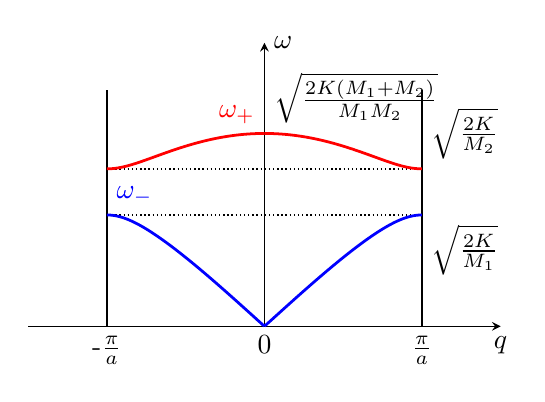
\begin{tikzpicture}
      [scale=2.0]
      \draw[->, >=stealth] (-1.5, 0.0) -- (1.5, 0.0) node[below] {$q$};
      \draw[->, >=stealth] (0.0, 0.0) -- (0.0, 1.8) node[right] {$\omega$};
      \node[below] at (0, 0) {0};

      \draw[line width=0.5pt] (1.0, 0.0) -- (1.0, 1.5);
      \draw[line width=0.5pt] (-1.0, 0.0) -- (-1.0, 1.5);
      % \draw[line width=0.5pt, densely dotted] (-1.0, 1.0) -- (1.0, 1.0);

      \node[below, align=left] at (1.0, 0.0) {${\pi\over a}$};
      \node[below, align=right] at (-1.0, 0.0) {-${\pi\over a}$};
      \node[right, anchor=south west] at (0.0, 1.2247448) {$\sqrt{2K(M_1+M_2)\over M_1M_2}$};
      \node[right, anchor=north west] at (1.0, 0.7071067) {$\sqrt{2K\over M_1}$};
      \node[right, anchor=south west] at (1.0, 1.0000000) {$\sqrt{2K\over M_2}$};

      \node[right, anchor=south west] at (-1.0, 0.7071067) {$\mathcolor{blue}{\omega_{-}}$};
      \node[left, anchor=south east] at (0.0, 1.2247448) {$\mathcolor{red}{\omega_{+}}$};

      \draw[line width=0.5pt, densely dotted] (-1.0, 1.0) -- (1.0, 1.0);
      \draw[line width=0.5pt, densely dotted] (-1.0, 0.7071067) -- (1.0, 0.7071067);

      % M1 = 1./3; M2 = 2./3; K = 1.5
      % optical modes
      \draw[line width=1.0pt, color=red, domain=0:1.0, solid] plot[samples=300]
      (\x, {sqrt(1./4*(3 + sqrt(5 + 4*cos(\x r * pi ))))});
      \draw[line width=1.0pt, color=red, domain=-1:.0, solid] plot[samples=300]
      (\x, {sqrt(1./4*(3 + sqrt(5 + 4*cos(\x r * pi ))))});
      % acoustic modes
      \draw[line width=1.0pt, color=blue, domain=0:1.0, solid] plot[samples=300]
      (\x, {sqrt(1./4*(3 - sqrt(5 + 4*cos(\x r * pi ))))});
      \draw[line width=1.0pt, color=blue, domain=-1:.0, solid] plot[samples=300]
      (\x, {sqrt(1./4*(3 - sqrt(5 + 4*cos(\x r * pi ))))});
    \end{tikzpicture}
  \end{center}
\end{frame}